% \AtBeginSection[]{
%     \begin{frame}
%         \frametitle{}
%         \tableofcontents[currentsection]
%     \end{frame}
% }

%%%%%%%%%%%%%%%%%%%%%%%%%%%%%%%%%%%%

\section{Fondements théoriques : MARL et MO}



\subsection{(G1) Apprentissage par Renforcement Multi-Agent}

% \begin{frame}{(G1) Apprentissage par Renforcement Multi-Agent}{Notions de base du MARL}

%     \begin{columns}

%         \hspace{-2ex}

%         \begin{column}{0.4\textwidth}

%             \begin{figure}
%                 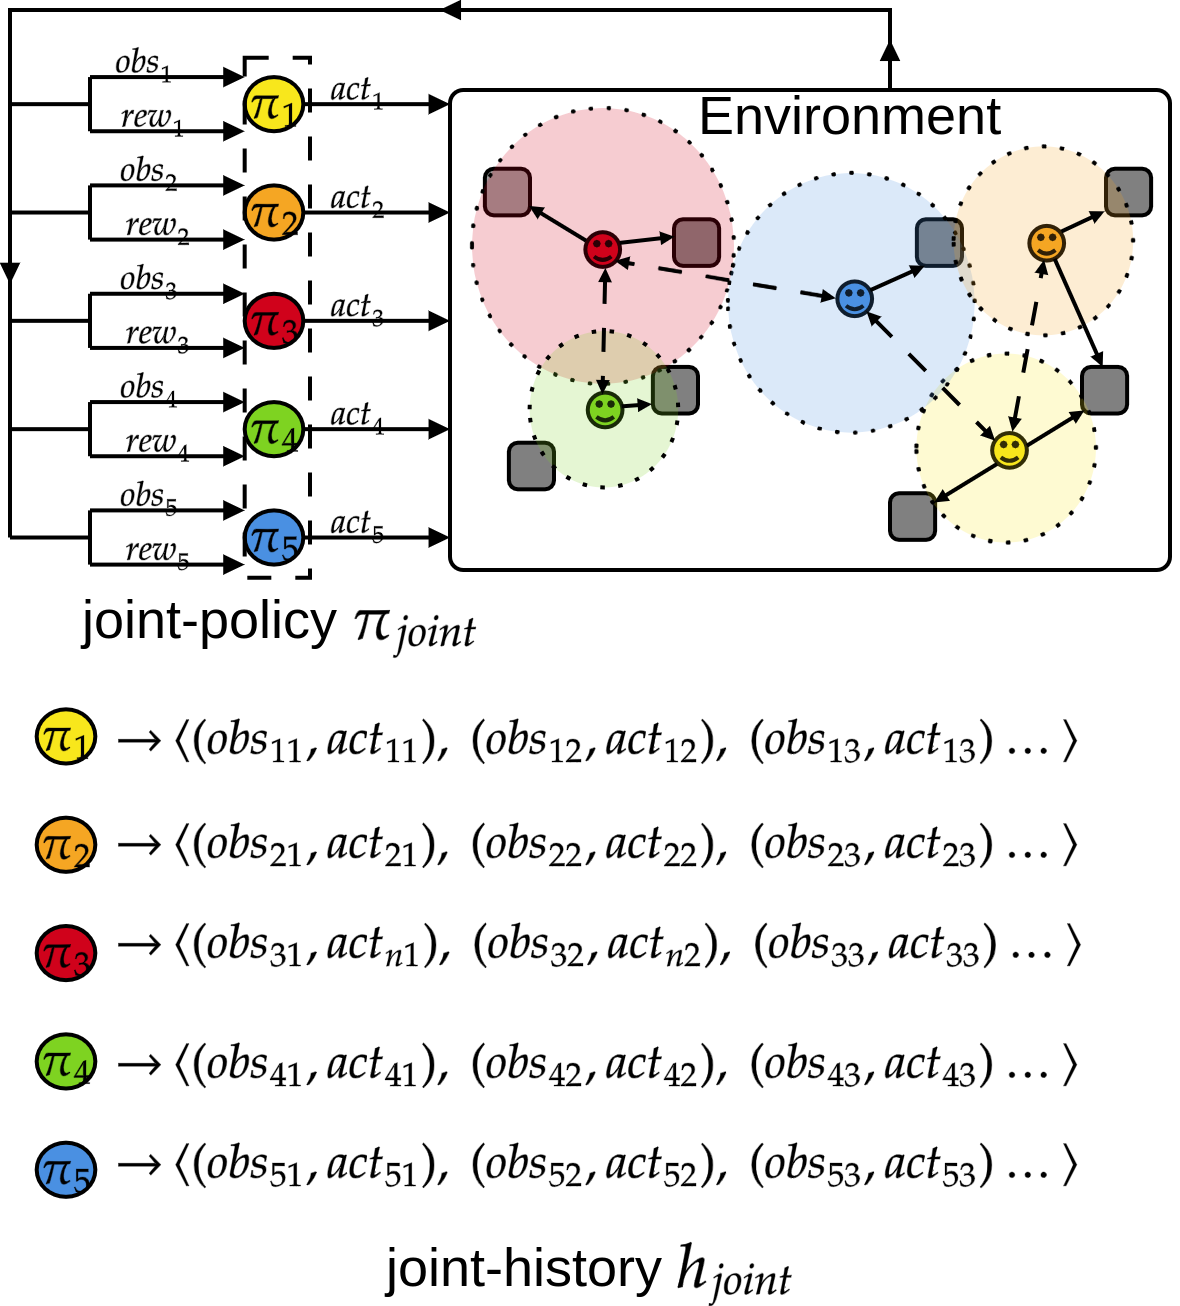
\includegraphics[width=\linewidth]{figures/marl_basics.png}
%             \end{figure}

%         \end{column}

%         \begin{column}{0.7\textwidth}
%             \vspace{-2ex}

%             \begin{center}
%                 \begin{minipage}{0.95\linewidth}
%                     \centering
%                     \begin{block}{Modèles markoviens pour le MARL : Dec-POMDP}
%                         {\small
%                             Processus de Décision Markovien Partiellement Observable Décentralisé (Dec-POMDP)~\cite{Oliehoek2016}
%                             \begin{itemize}
%                                 \item considère plusieurs agents dans un style SMA similaire;
%                                 \item processus stochastiques pour l'incertitude dans les changements d'environnement, y compris les observations;
%                                 \item la fonction de récompense est commune aux agents, ce qui favorise l'entraînement pour des actions orientées vers la collaboration~\cite{Beynier2013}
%                             \end{itemize}
%                         }
%                         \

%                         { \scriptsize

%                         $(S,\{A_i\},T,R,\{\Omega_i\},O,\gamma)$ , où
%                         \begin{itemize}
%                             \item $S = \{s_1, ..s_{|S|}\}$ : L'ensemble des états possibles;
%                             \item $A_{i} = \{a_{1}^{i},..,a_{|A_{i}|}^{i}\}$ : L'ensemble des actions possibles pour l'agent $i$;
%                             \item $T$ tel que $T(s,a,s') = \probP{(s'|s,a)}$ : L'ensemble des probabilités de transition conditionnelles;
%                             \item $R: S \times A \times S \rightarrow \mathbb{R}$ : La fonction de récompense;
%                             \item $\Omega_{i} = \{o_{1}^{i},..,o_{|\Omega_{i}|}^{i}\}$ : L'ensemble des observations pour l'agent $ag_i$;
%                             \item $O$ tel que $O(s',a,o) = \probP{(o|s',a)}$ : L'ensemble des probabilités d'observation conditionnelles;
%                             \item $\gamma \in [0,1]$, le facteur de discount.
%                         \end{itemize}

%                         }

%                     \end{block}

%                 \end{minipage}
%             \end{center}

%         \end{column}

%     \end{columns}

% \end{frame}

\begin{frame}{(G1) Apprentissage par Renforcement Multi-Agent}{MARL pour la résolution/conception}

    \begin{block}{MARL pour un usage méthodologique dans la littérature ?}

        Politiques conjointes efficaces mais \textbf{non explicitement} spécifiées/compréhensibles
        $\Longrightarrow$ Peu de travaux relatifs
            {\small
                \begin{itemize}
                    \item Kazhdan et al.~\cite{Kazhdan2020} ont proposé des moyens d'extraire des modèles symboliques $\rightarrow$ \textbf{pas évolutif};
                    \item Wang et al.~\cite{Wang2020} : ont introduit une approche MARL orientée rôle $\rightarrow$ \textbf{uniquement les rôles};
                    \item Zheng et al.~\cite{Zheng2018} ont présenté une plateforme pour le MARL $\rightarrow$ \textbf{outils empiriques}.
                \end{itemize}
            }
    \end{block}

    \begin{block}{Formalisation et Résolution un Dec-POMDP}

        \begin{itemize}
            \item \textbf{Dec-POMDP} : récompense commune $\rightarrow$ favorise coopération (vs. POSG) ;
            \item \textbf{résolution} : trouver une politique conjointe $\pi_{joint,i} \in \Pi_{joint}$ de sorte que la récompense cumulative espérée dans le temps soit au moins $s \in \mathbb{R}$.
        \end{itemize}


    \end{block}

    \begin{exampleblock}{Algorithmes favorisés MARL}
        {\footnotesize

            \centering
            \begin{minipage}{0.5\textwidth}
                \centering
                \begin{itemize}
                    \item \textbf{Entraînement Centralisé, Exécution Décentralisée} : MADDPG, COMA
                \end{itemize}
            \end{minipage}\hfill
            \begin{minipage}{0.5\textwidth}
                \centering
                \begin{itemize}
                    \item \textbf{MARL Coopératif} : QMIX, MAPPO
                \end{itemize}
            \end{minipage}\hfill
        }
    \end{exampleblock}

\end{frame}

\subsection{Modèle Organisationnel}

\begin{frame}{(G2) Modèle Organisationnel}{$\mathcal{M}OISE^+$}

    \begin{figure}
        \centering
        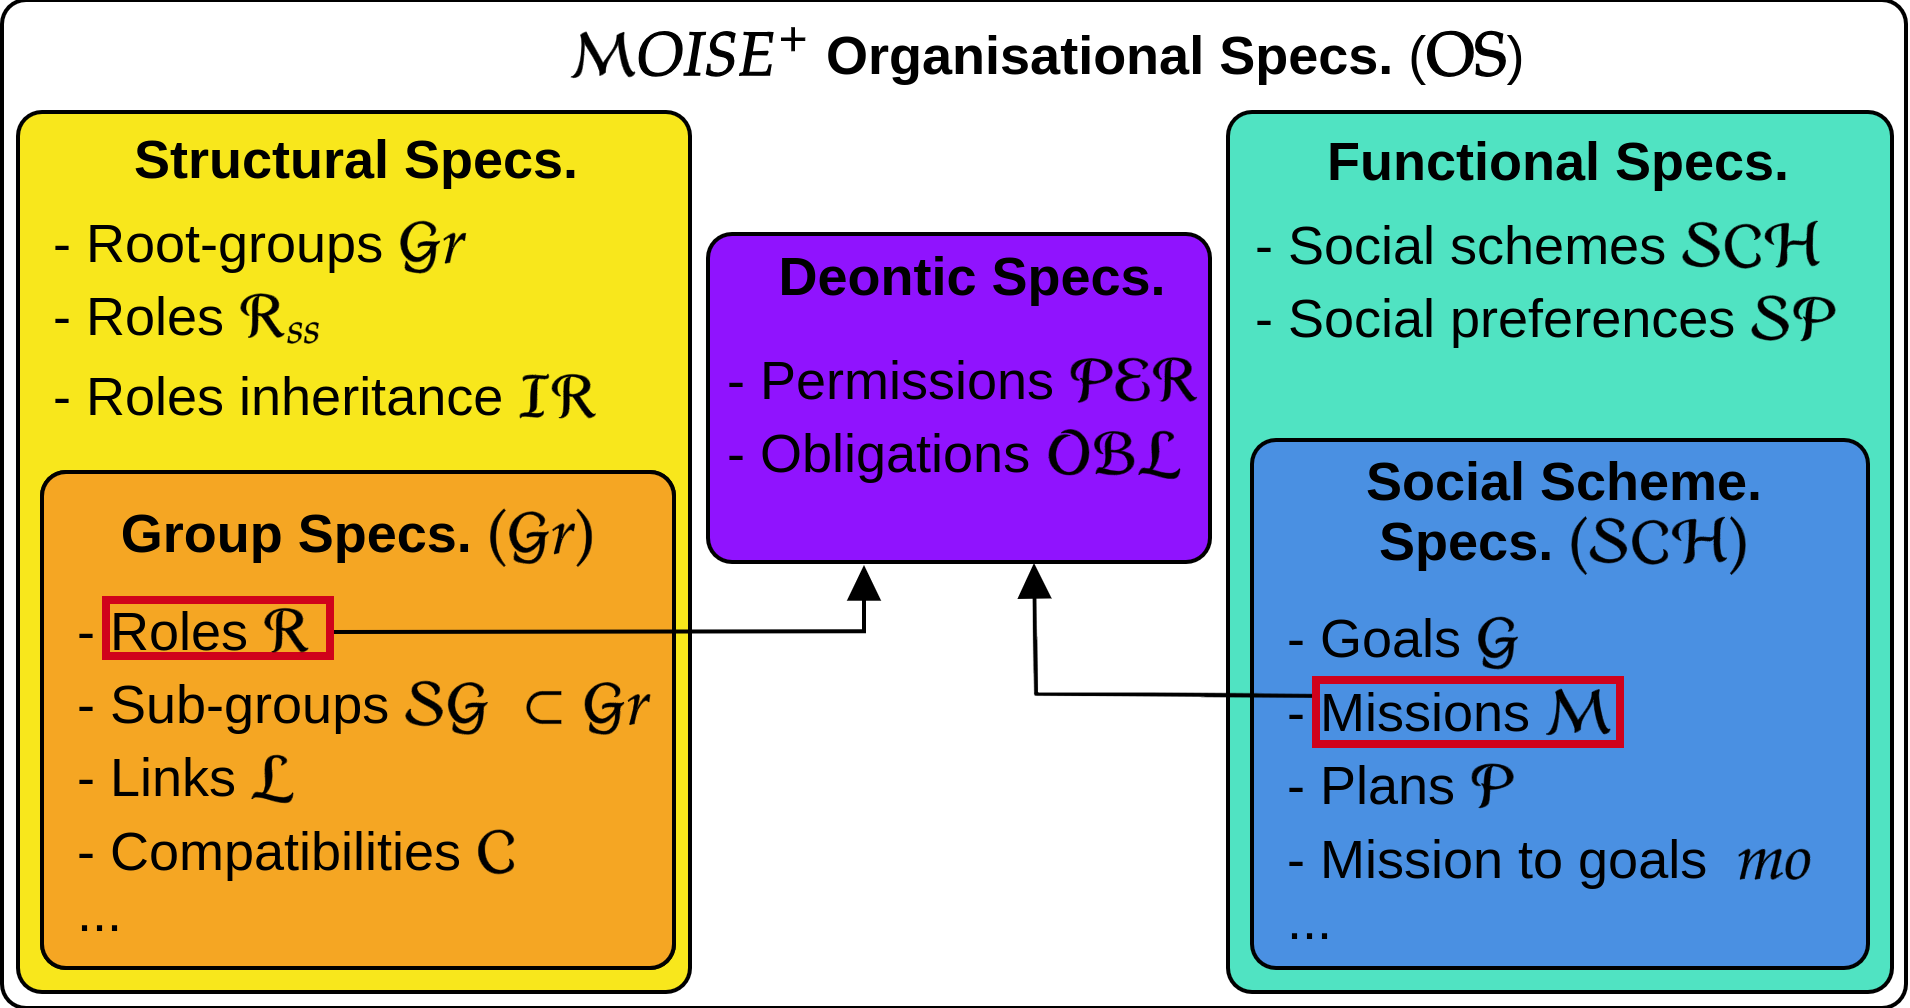
\includegraphics[width=0.75\linewidth]{figures/moise_model.png}
    \end{figure}

    \begin{spacing}{0.25}
        {\tiny Hübner, J. F., Sichman, J. S., et Boissier, O. (2002).
            Un modèle pour la spécification structurelle, fonctionnelle et déontique
            des organisations dans les systèmes multiagents.
            Dans Bittencourt, G. et Ramalho, G. L., éditeurs, Actes du 16e Symposium Brésilien d'Intelligence Artificielle (SBIA’02), volume 2507 de LNAI, pages 118–128, Berlin. Springer.}
    \end{spacing}

\end{frame}

% \begin{frame}{(G2) Modèle Organisationnel}{\textit{Exemple d'équipe de football}}

%     \vspace{-2.5ex}

%     \begin{columns}
%         \hspace{-16ex}
%         \begin{column}{0.5\textwidth}
%             \centering
%             \begin{figure}[H]
%                 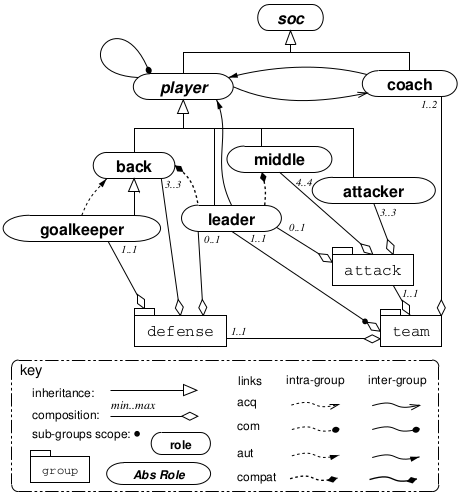
\includegraphics[width=0.7\textwidth]{figures/soccer_ss.png}
%                 \caption*{Spécifications Structurelles}
%             \end{figure}
%         \end{column}
%         \hspace{-20ex}
%         \begin{column}{0.5\textwidth}
%             \centering
%             \begin{figure}[H]
%                 \centering
%                 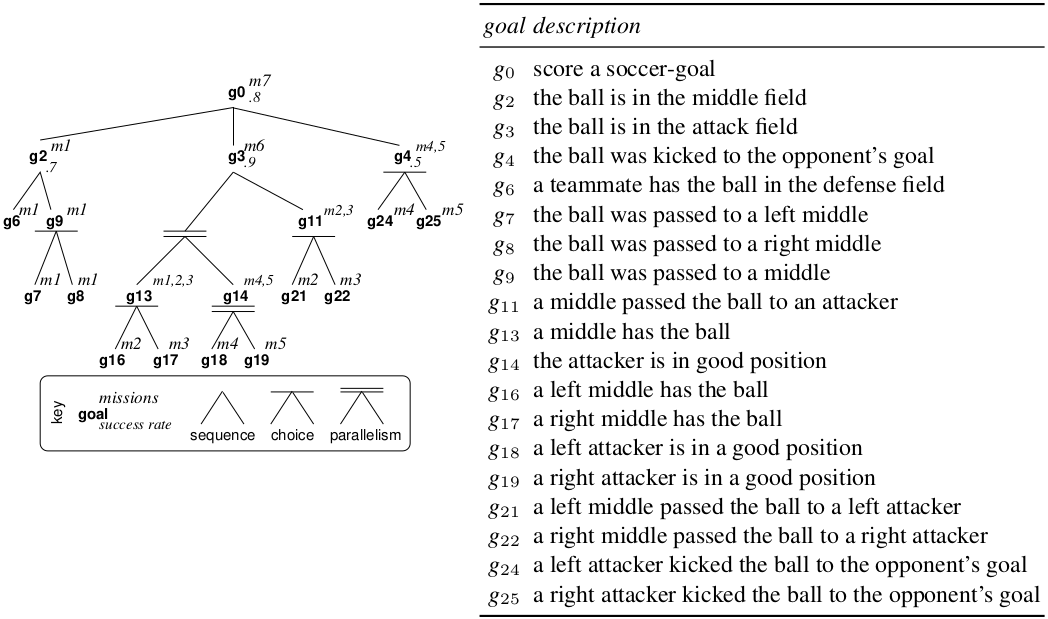
\includegraphics[width=1.2\textwidth]{figures/soccer_fs.png}
%                 \caption*{Spécifications Fonctionnelles}
%             \end{figure}
%         \end{column}
%     \end{columns}

%     \ \\

%     \begin{minipage}{\textwidth}
%         \centering
%         \begin{figure}[H]
%             \centering
%             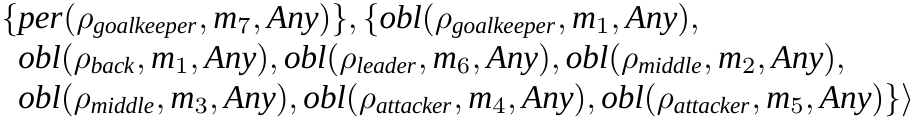
\includegraphics[width=0.4\linewidth]{figures/soccer_ds.png}
%             \caption*{Spécifications Déontiques}
%         \end{figure}
%     \end{minipage}

% \end{frame}


\subsection{$\mathcal{M}OISE^+$ et MARL}

\begin{frame}{$\mathcal{M}OISE^+$ et MARL}{Aperçu}

    \begin{block}{MARL orienté organisation (OMARL)}
        Un processus de MARL enrichi d'un modèle organisationnel pour :
        \begin{itemize}
            \item \textbf{Contraindre l'espace des politiques} satisfaisant les spécifications de conception données ;
            \item \textbf{Inférer les spécifications organisationnelles} à partir des politiques des agents.
        \end{itemize}
    \end{block}

    \begin{block}{\emph{Partial Relations with Agents' History and Organizational Model} (PRAHOM)}
        Mise en oeuvre d'un processus OMARL\dots
        \begin{enumerate}
            \item \textbf{Contraindre l'espace des politiques}
                  \begin{itemize}
                      \item Impossible d'utiliser directement les politiques $\rightarrow$ \textbf{historiques} caractérisant les \textbf{politiques} ;
                      \item Relations entre \textbf{SO} et les \textbf{historiques} attendus ;
                      \item A chaque iteration, changement de l'espace des actions et récompenses pour appliquer les \textbf{SO} en MARL.
                  \end{itemize}

            \item \textbf{Inférer les spécifications organisationnelles}
                  \begin{itemize}
                      \item Analyser les historiques $\rightarrow$ caractériser les comportements collectifs en tant que SO ;
                      \item Utiliser les relations connues entre les SO et les historiques ;
                      \item Utiliser la définition générale des SO par rapport aux historiques.
                  \end{itemize}
        \end{enumerate}
    \end{block}
\end{frame}




